\subsection{Logic-Quellpaket}
    \subsubsection{GUIConnector}
        \begin{table}[H]
            \caption{Interface GUIConnector}
            \begin{tabular}{p{2.5cm}  p{9.5cm}} 
                \hline
                \textbf{Eigenschaft} & \textbf{Beschreibung}\\
                \hline
                Name & GUIConnector\\
                Ort & Quellpaket \textit{logic}\\
                \hline
                Zweck &
                Das Interface bildet, durch vorgegebene Methoden, eine Schnittstelle zwischen der Logik und der graphischen Oberfläche.
                Die Klassen \textit{JavaFxGUI} und \textit{FakeGui} implementieren dieses Interface.
                \\
                \hline
                Struktur &
                \begin{itemize}
                    \itemsep0em
                    \item Bietet eine Schnittstelle zur Manipulation der graphischen Elemente
                    \item Fordert alle Unterklassen alle Methoden zu implementieren
                \end{itemize}
                \\
                \hline
            \end{tabular}
        \end{table}

        \begin{figure}[H]
            \centering
            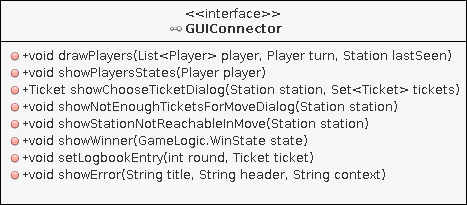
\includegraphics[scale=0.7]{img/uml/guiConnector.png}   
            \caption{GUIConnector UML-Klassendiagramm}
        \end{figure}



    \subsubsection{GameLogic}
        \begin{table}[H]
            \caption{Klasse GameLogic}
            \begin{tabular}{p{2.5cm}  p{9.5cm}} 
                \hline
                \textbf{Eigenschaft} & \textbf{Beschreibung}\\
                \hline
                Name & GameLogic\\
                Ort & Quellpaket \textit{logic}\\
                \hline
                Zweck &
                Verwaltet alle nötigen Spielelemente und lässt diese miteinander interagieren.
                Des Weiteren werden Benutzereingaben vom \textit{FXMLDocumentController}, wie ein Klicken auf ein Element in der graphischen Oberfläche,
                an die \textit{GameLogic} delegiert um dort verarbeitet zu werden.
                \\
                \hline
                Struktur &
                \begin{itemize}
                    \itemsep0em
                    \item Hält eine statische Klasse \textit{Config} in der alle wichtigen Konstanten abgelegt sind
                    \item Verwaltet das Spielfeld in einer \textit{Board}-Instanz
                    \item Verwaltet eine Gruppe an Detektiven in mehreren \textit{Detective}-Instanzen und Mister-X in einer \textit{MisterX}-Istanz
                    \item Nimmt Benutzereingaben entgegen und verarbeitet diese ihren \textit{handler}-Methoden
                    \item Ein Spiel kann über einen speziellen Konstruktor geladen werden
                    \item Regelt den Ablauf zwischen jedem Zug und steuert die KI der einzelnen Spieler
                    \item Hält zusätzliche Informationen über das Spiel wie die Spielrunde oder wer aktuell dran ist
                \end{itemize}
                \\
                \hline
            \end{tabular}
        \end{table}
        \begin{figure}[H]
            \centering
            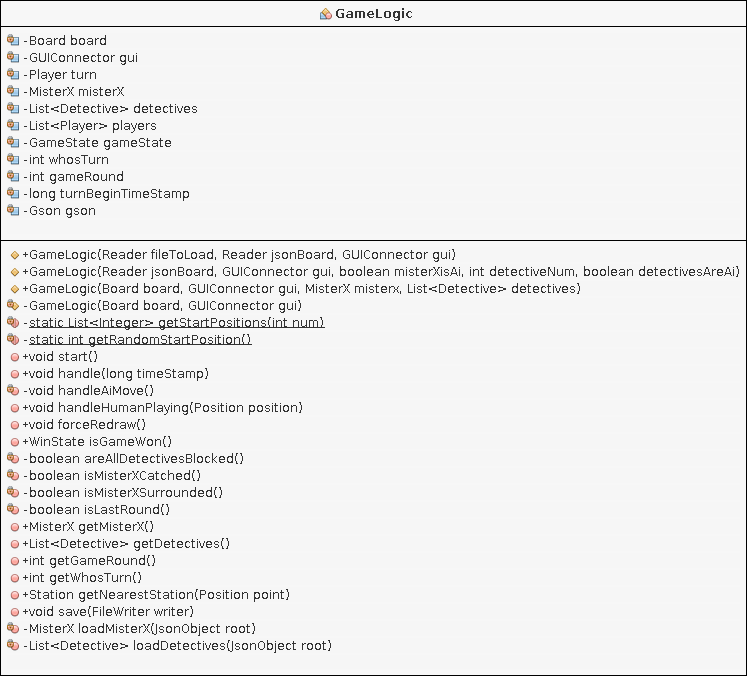
\includegraphics[scale=0.5]{img/uml/gameLogic.png}   
            \caption{GameLogic UML-Klassendiagramm}
        \end{figure}


    \subsubsection{Move}
        \begin{table}[H]
            \caption{Klasse Move}
            \begin{tabular}{p{2.5cm}  p{9.5cm}} 
                \hline
                \textbf{Eigenschaft} & \textbf{Beschreibung}\\
                \hline
                Name & Move\\
                Ort & Quellpaket \textit{logic}\\
                \hline
                Zweck &
                Repräsentiert einen Zug innerhalb des Netzes.
                \\
                \hline
                Struktur &
                \begin{itemize}
                    \itemsep0em
                    \item Hält eine \textit{Station}-Instanz die das Ziel des Zuges repräsentiert
                    \item Hält ein \textit{Ticket}-Wert der das Ticket für den Zug wiederspiegelt
                \end{itemize}
                \\
                \hline
            \end{tabular}
        \end{table}
        \begin{figure}[H]
            \centering
            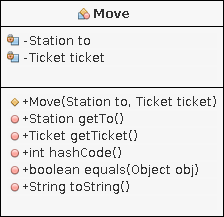
\includegraphics[scale=0.7]{img/uml/move.png}   
            \caption{Move UML-Klassendiagramm}
        \end{figure}


    \subsubsection{Ticket}
        \begin{table}[H]
            \caption{Klasse Ticket}
            \begin{tabular}{p{2.5cm}  p{9.5cm}} 
                \hline
                \textbf{Eigenschaft} & \textbf{Beschreibung}\\
                \hline
                Name & Ticket\\
                Ort & Quellpaket \textit{logic}\\
                \hline
                Zweck &
                Bildet die Tickets für die verschiedenen Verkehrsmittel ab.
                \\
                \hline
                Struktur &
                \begin{itemize}
                    \itemsep0em
                    \item Hält die Enumkonstanten \textit{CAB, BUS, TUBE, BLACK}
                    \item bietet über die \textit{from}-Methode eine Möglichkeit über einen Ordinalwert ein Ticket zu generieren
                \end{itemize}
                \\
                \hline
            \end{tabular}
        \end{table}
        \begin{figure}[H]
            \centering
            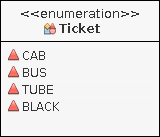
\includegraphics[scale=0.7]{img/uml/ticket.png}   
            \caption{Ticket UML-Klassendiagramm}
        \end{figure}


